\subsection*{Appendix D}

This appendix provides supporting descriptive statistics to aid interpretation of the marginal effects presented in GAM analysis. Since GAM marginal effects were estimated at specific percentiles of key continuous variables, in Tables~\ref{tab:quantiles_orlando_c} and \ref{tab:quantiles_orlando_e} I report the corresponding values for those percentiles in the Central and East Orlando datasets, respectively. These values contextualize how attribute levels vary across the distributions. For instance, in Central Orlando, the number of bathrooms equals 2 at the $10^{\text{th}}$, $25^{\text{th}}$, and $50^{\text{th}}$ percentiles, which helps explain the marginal effects reported at those points: since the value of the variable does not change across these percentiles, the model captures little variation in price response, resulting in misleading negative estimated effects.

Figures (a) through (l) plot the smoothed effects of the six continuous covariates on the logarithm of sale price for Central and East Orlando. Together with the percentile values, the curves reveal consistent and interpretable patterns. 

Central Orlando shows a distinct nonlinear relationship between property age and prices, with values declining until the median age (approximately 42 years), then rising for very old homes. East Orlando’s newer housing stock (with a median age of 27 years) displays a mostly downward slope with only a slight uptick beyond about 60 years --- a range populated by fewer than 10 percent of observations. Hence, the marginal effects at high percentiles differ significantly across the two regions.

\begin{table}
\caption{Quantiles of Continuous Variables in Orlando Central Dataset}
\label{tab:quantiles_orlando_c}
\begin{tabular}{lccccc}
\toprule
 & 10\% & 25\% & 50\% & 75\% & 90\% \\
\midrule
age & 17.00 & 31.00 & 42.00 & 59.00 & 68.00 \\
bedrooms & 2.00 & 2.00 & 3.00 & 3.00 & 4.00 \\
bathrooms & 2.00 & 2.00 & 2.00 & 3.00 & 3.00 \\
sqft\_per\_bedroom & 377.33 & 430.67 & 500.00 & 586.67 & 686.33 \\
avg\_schools\_rating & 3.67 & 4.00 & 4.33 & 4.67 & 5.33 \\
min\_distance\_highway & 0.57 & 1.01 & 1.59 & 2.22 & 2.74 \\
\bottomrule
\end{tabular}
\end{table}


\begin{table}
\caption{Quantiles of Continuous Variables in Orlando East Dataset}
\label{tab:quantiles_orlando_e}
\begin{tabular}{lccccc}
\toprule
 & 10\% & 25\% & 50\% & 75\% & 90\% \\
\midrule
age & 6.00 & 19.00 & 27.00 & 37.00 & 43.00 \\
bedrooms & 3.00 & 3.00 & 3.00 & 4.00 & 4.00 \\
bathrooms & 2.00 & 2.00 & 2.00 & 3.00 & 3.00 \\
sqft\_per\_bedroom & 401.09 & 468.50 & 530.00 & 614.00 & 701.30 \\
avg\_schools\_rating & 4.00 & 4.33 & 5.00 & 5.67 & 6.00 \\
min\_distance\_highway & 0.54 & 1.01 & 1.96 & 3.79 & 4.92 \\
\bottomrule
\end{tabular}
\end{table}




In both markets, additional bedrooms are valued, but the slope is steeper in Central Orlando. Moving from four to six bedrooms raises the logarithm of price by roughly 0.9 in Central Orlando versus 0.4 in East Orlando, reflecting the premium for large homes near the urban core. Bathrooms also show different dynamics: in Central Orlando the curve is peaking around five to six bathrooms and then flattens out, while in East Orlando the effect increases steadily across the range, consistent with newer construction and larger lot sizes. The \texttt{sqft\_per\_bedroom} variable shows positive but diminishing returns in both regions. 

The \texttt{avg\_schools\_rating} is generally higher in East Orlando across all percentiles, reflecting better average school quality in suburban areas. Central Orlando’s effect rises quickly from the $10^{\text{th}}$ to the $60^{\text{th}}$ percentile, then levels off, showing that school quality is important, but its marginal contribution diminishes once ratings exceed “good.” East Orlando shows a nearly linear gain over the entire observed range, likely because higher ratings are both attainable and less correlated with neighborhood age or density. As a result, the marginal effects at common percentiles are uniformly positive and somewhat larger in the East.

The \texttt{min\_distance\_highway} values are notably larger in East Orlando, consistent with the region’s more dispersed layout and greater distance from major transportation corridors. In Central Orlando, proximity to the highway carries a premium, after which the effect declines --- buyers value quick access but tend to discount properties that are several miles out. In East Orlando, the pattern is reverse: prices are slightly lower within roughly one mile of an exit (likely due to noise and traffic), then rise steadily out to seven miles, capturing the convenience–disamenity trade‑off in the suburb.

This analysis underscores that the same physical attribute can influence price in different, nonlinear ways across sub‑markets. Presenting both the percentile tables and the GAM curves makes these location‑specific nonlinearities transparent, thereby improving the interpretability of the flexible GAM specification for practitioners and policy analysts alike.



\begin{figure}[H]
  \centering
  % left graphic ----------------------------------------------------
  \begin{minipage}[t]{0.48\textwidth}
    \centering
    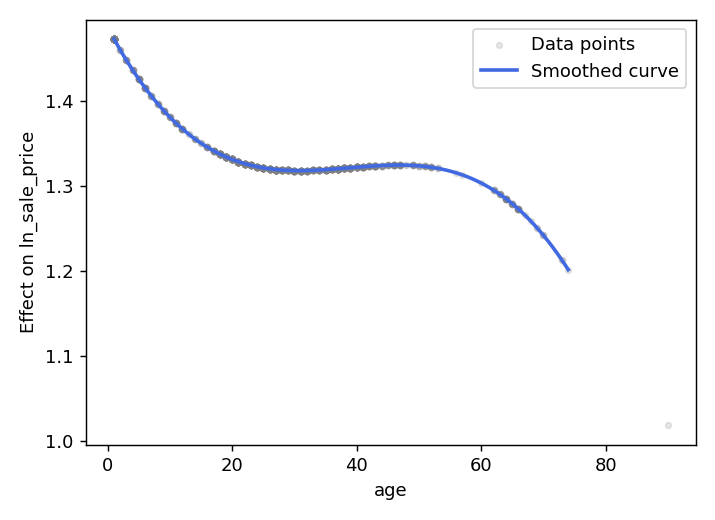
\includegraphics[width=\linewidth]{Figures/orlando_east_age_smooth.png}
    \caption*{\small (a) GAM smooth for age (Orlando East)}
  \end{minipage}
  \hfill
  % right graphic ---------------------------------------------------
  \begin{minipage}[t]{0.48\textwidth}
    \centering
    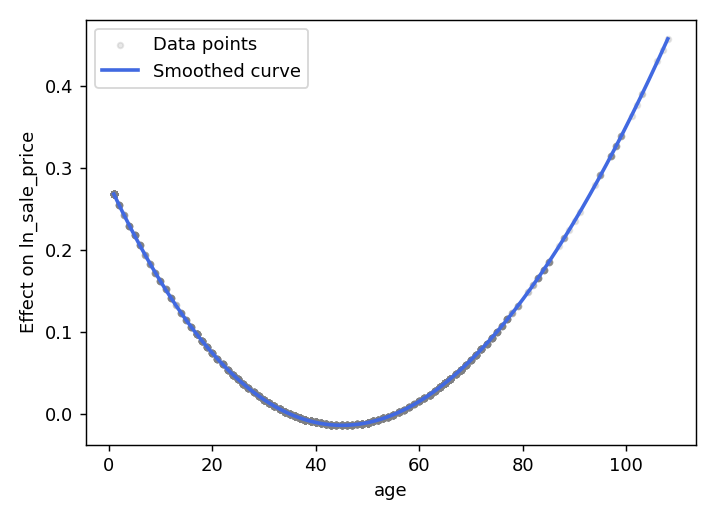
\includegraphics[width=\linewidth]{Figures/orlando_central_age_smooth.png}
    \caption*{\small(b) GAM smooth for age (Orlando Central)}
  \end{minipage}
\end{figure}


\begin{figure}[H]
  \centering
  \begin{minipage}[t]{0.48\textwidth}
    \centering
    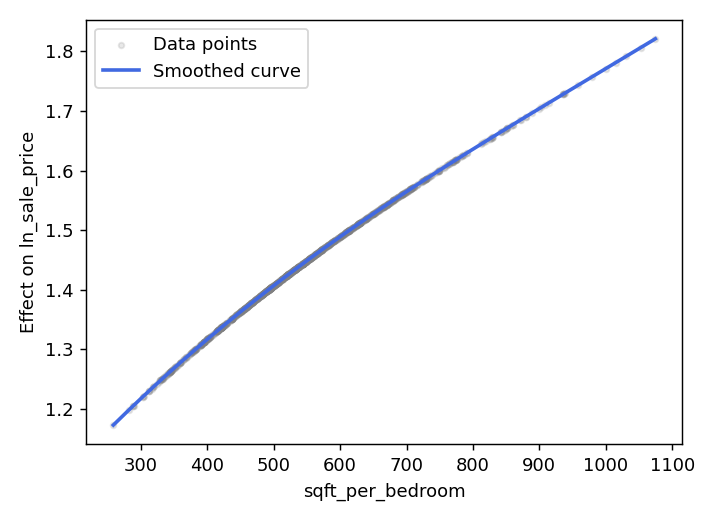
\includegraphics[width=\linewidth]{Figures/orlando_east_sqft_per_bedroom_smooth.png}
    \caption*{\small \centering (c) GAM smooth for sqft per bedroom \par (Orlando East)}
  \end{minipage}
  \hfill
  \begin{minipage}[t]{0.48\textwidth}
    \centering
    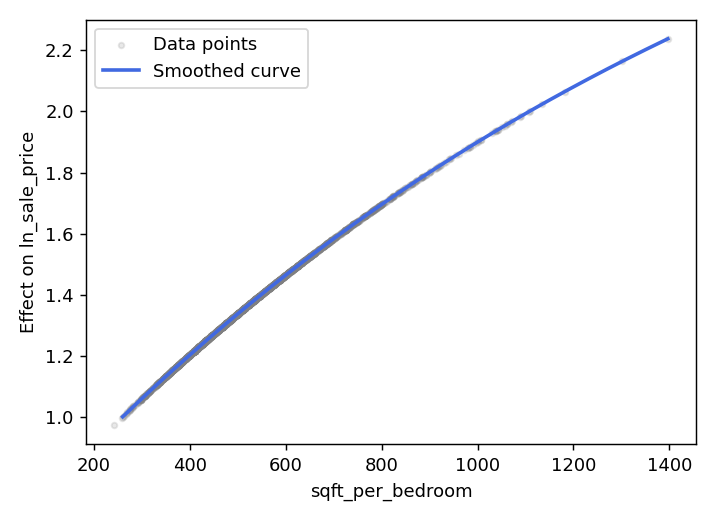
\includegraphics[width=\linewidth]{Figures/orlando_central_sqft_per_bedroom_smooth.png}
    \caption*{\small \centering (d) GAM smooth for sqft per bedroom \par (Orlando Central)}
  \end{minipage}
\end{figure}



\begin{figure}[H]
  \centering
  % left graphic ----------------------------------------------------
  \begin{minipage}[t]{0.48\textwidth}
    \centering
    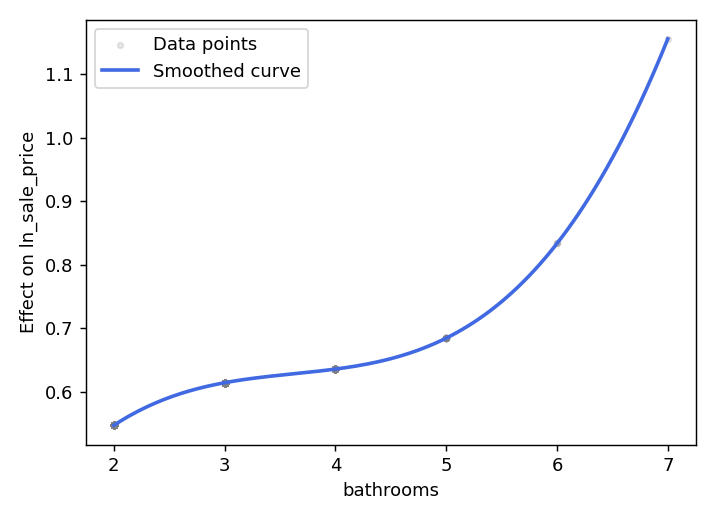
\includegraphics[width=\linewidth]{Figures/orlando_east_bathrooms_smooth.png}
    \caption*{\small(e) GAM smooth for bathrooms (Orlando East)}
  \end{minipage}
  \hfill
  % right graphic ---------------------------------------------------
  \begin{minipage}[t]{0.48\textwidth}
    \centering
    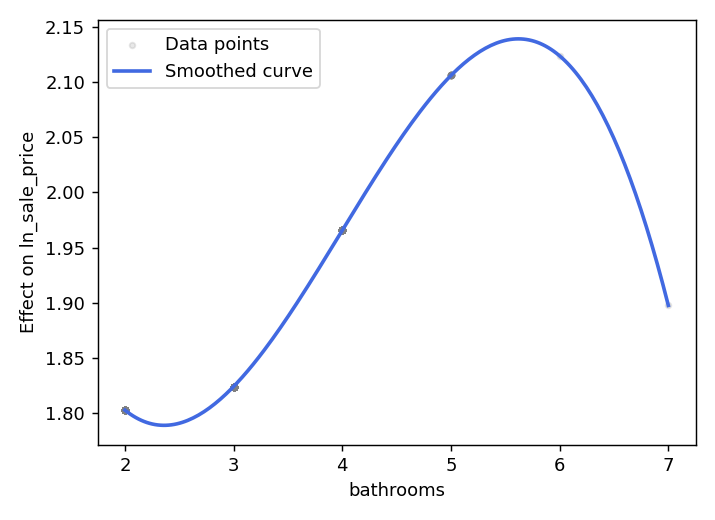
\includegraphics[width=\linewidth]{Figures/orlando_central_bathrooms_smooth.png}
    \caption*{\small(f) GAM smooth for bathrooms (Orlando Central)}
  \end{minipage}
\end{figure}

\begin{figure}[H]
  \centering
  \begin{minipage}[t]{0.48\textwidth}
    \centering
    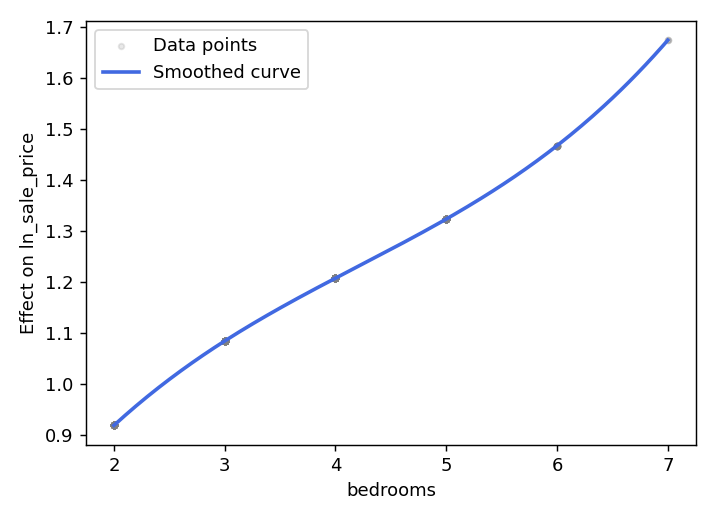
\includegraphics[width=\linewidth]{Figures/orlando_east_bedrooms_smooth.png}
    \caption*{\small(g) GAM smooth for bedrooms (Orlando East)}
  \end{minipage}
  \hfill
  \begin{minipage}[t]{0.48\textwidth}
    \centering
    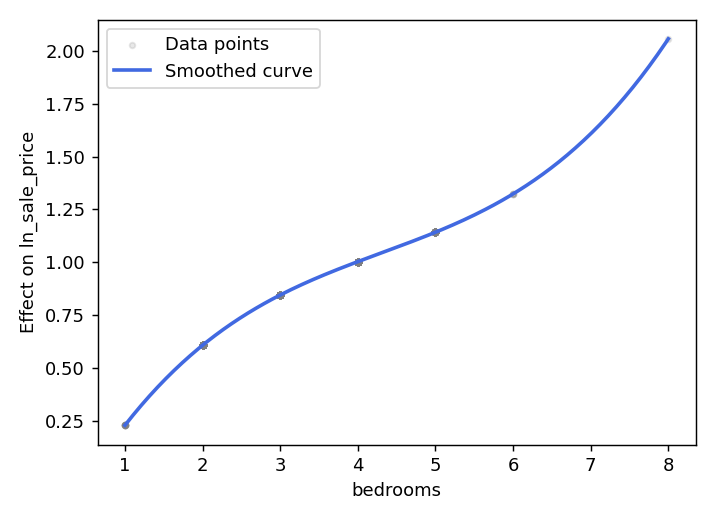
\includegraphics[width=\linewidth]{Figures/orlando_central_bedrooms_smooth.png}
    \caption*{\small (h) GAM smooth for bedrooms (Orlando Central)}
  \end{minipage}
\end{figure}


\begin{figure}[H]
  \centering
  \begin{minipage}[t]{0.48\textwidth}
    \centering
    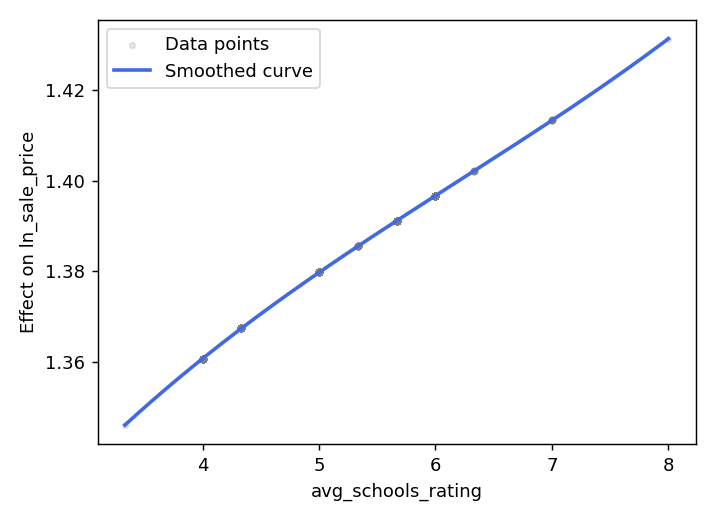
\includegraphics[width=\linewidth]{Figures/orlando_east_avg_schools_rating_smooth.png}
    \caption*{\small \centering (i) GAM smooth for school rating \par (Orlando East)}
  \end{minipage}
  \hfill
  \begin{minipage}[t]{0.48\textwidth}
    \centering
    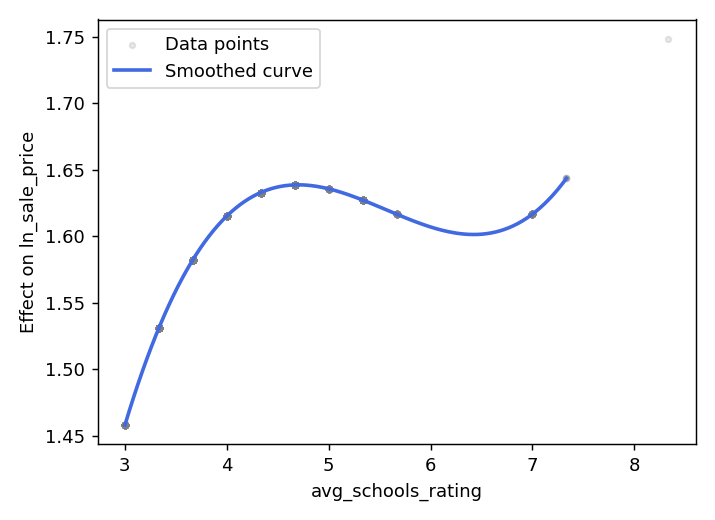
\includegraphics[width=\linewidth]{Figures/orlando_central_avg_schools_rating_smooth.png}
    \caption*{\small \centering (j) GAM smooth for school rating \par (Orlando Central)}
  \end{minipage}
\end{figure}


\begin{figure}[H]
  \centering
  \begin{minipage}[t]{0.48\textwidth}
    \centering
    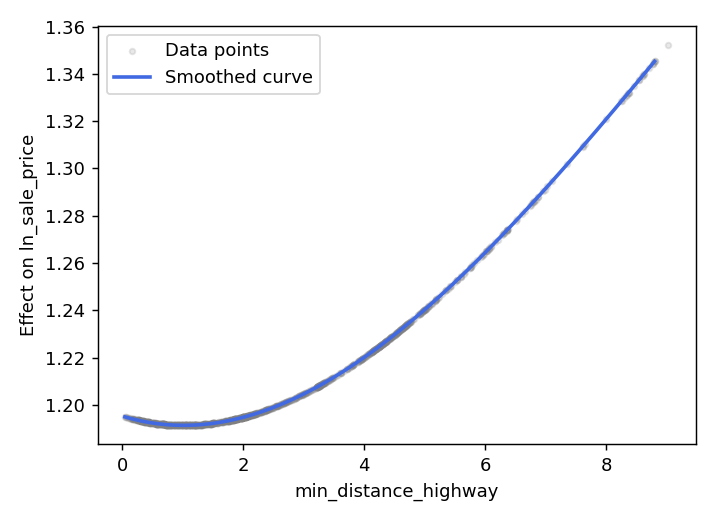
\includegraphics[width=\linewidth]{Figures/orlando_east_min_distance_highway_smooth.png}
    \caption*{\small \centering (k) GAM smooth for min distance to highway \par(Orlando East)}
  \end{minipage}
  \hfill
  \begin{minipage}[t]{0.48\textwidth}
    \centering
    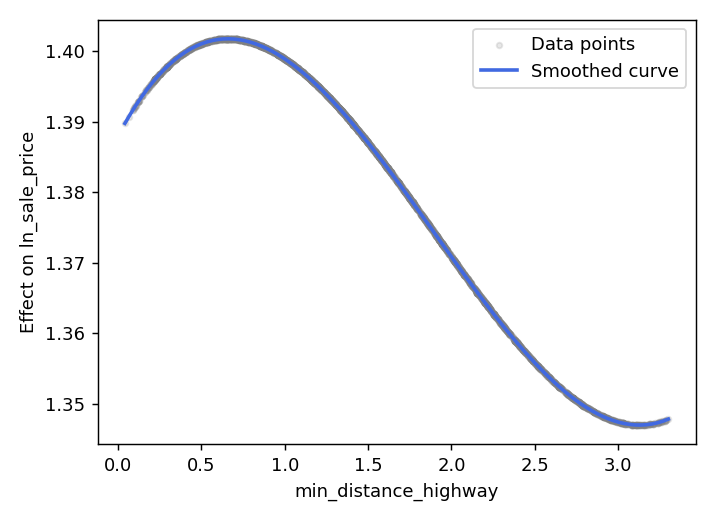
\includegraphics[width=\linewidth]{Figures/orlando_central_min_distance_highway_smooth.png}
    \caption*{\small \centering (l) GAM smooth for min distance to highway \par(Orlando Central)}
  \end{minipage}
\end{figure}


\clearpage

